\documentclass[specialist, subf, href, colorlinks=true, 14pt, times, mtpro, final]{disser}

\usepackage[utf8x]{inputenc}
\usepackage[english, russian]{babel}
\usepackage[T2A]{fontenc}
\usepackage{amsmath,amsthm,amssymb}
\usepackage {wrapfig}
\usepackage {enumitem}  
\usepackage{graphicx}
\usepackage{multicol}
\usepackage{mathrsfs}
\usepackage{xcolor}
\usepackage{hyperref}
\usepackage{tikz}
\usepackage{pdfpages}


\usetikzlibrary{decorations.pathreplacing}
\usepackage[noend]{algpseudocode}
\usepackage[a4paper, mag=1000, includefoot, left=1.5cm, right=1.5cm, top=1cm, bottom=1cm, headsep=1cm, footskip=1cm]{geometry}
\usepackage{floatrow}
\usepackage{tikz}
\newcommand{\RNumb}[1]{\uppercase\expandafter{\romannumeral #1\relax}}
\usetikzlibrary{graphs}

\theoremstyle{definition}
\newtheorem{defn}{Определение}[section]
\newtheorem{example}{Пример}[section]
\newtheorem{state}{Утверждение}[section]
\newtheorem{theorem}{Теорема}[section]
\newtheorem{lemma}{Лемма}[section]
\newtheorem{axiom}{Аксиома}[section]
\newtheorem{consequence}{Следствие}[section]

\begin{document}
	
	\begin{titlepage}
		\begin{center}
			
			Федеральное государственное бюджетное образовательное учреждение высшего образования 
			<<Московский Государственный Университет им.\,М.\,В.\,Ломоносова>>\\
			
			Механико-математический факультет
			
			\begin{figure}[!htp]
				\begin{center}
					{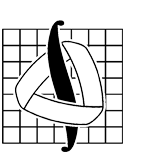
\includegraphics[width=20mm]{mmlogo.png}}
				\end{center}
			\end{figure}
			
			\vspace{3cm}
			
			Реферат по истории математики\\
			{\bf Основание топологии Анри Пуанкаре в цикле статей <<Analysis situs>>}
			
			\vspace{10cm}
			\begin{flushright}
				{\bfРаботу выполнил:}\\
				студент 4 курса Сибгатуллин Артур Петрович\\[0.5cm]
			\end{flushright}
			\vspace{1cm}
			
			\normalsize Москва, 2022
		\end{center}
	\end{titlepage}
	
	
	\tableofcontents
	
	\section{Введение}
	Об Анри Пуанкаре я узнал на первом курсе Механико-Математического факультета, для меня это был прежде всего не великий ученый, а автор "Гипотезы Пуанкаре". Однако после курса Дифференциальной Геометрии появилось желание познакомиться ближе с работами данного математика и его идеями, поэтому я выбрал данную тему для реферата по Истории математики.
	
	Основной используемой книгой для данного реферата была <<Пуанкаре А. Избранные труды>>  в трёх томах (Москва: Издательство <<Наука>>, 1971-1974. - Серия <<Классикинауки>>). Под редакцией Н.Н. Боголюбова\footnote{Боголюбов, Николай Николаевич, 1909-1992. Русский советский математик и физик-теоретик, академик АН СССР и АН УССР и проч.} , В.И. Арнольда\footnote{Арнольд, Владимир Игоревич, 1937-2010. Советский и российский математик, академик АН СССР и проч.} , И.Б. Погребысского\footnote{Погребысский, Иосиф Бенедиктович
	, 1906-1971. Советский математик, историк науки. д.ф.-м.н} . Книга является переводом избранных работ Пуанкаре, причем
	
	
	\newpage
	\begin{thebibliography}{100}
		\bibitem{Practicum} Численное моделирование нестационарного течения газа с использованием неявных разностных схем, \emph{Попов А.В., 2022}
		
	\end{thebibliography}
	
	
\end{document}
